% !TeX root = ../../../book.tex
\subsection{高斯驾到}\label{sec:section1.4.2}

\subsubsection*{问题描述}

在数学界有一个广为流传的轶事,可能是杜撰的,也可能是真实的,但很多人愿意相信它是真的,因为它的主角是有史以来最伟大的数学家/物理学家之一 --- 卡尔·弗里德里希·高斯(Carl Friedrich Gauss)。高斯活跃在 18 世纪末和 19 世纪初期至中期,并在很多领域证明了一些基本而有力的成果。他研究了数论、复分析、光学、几何、天文学等等! 阅读下面的故事,思考在这种情况下你会怎么做 --- 无论是小时候还是现在 --- 然后继续阅读进行讨论。

\begin{quote}
    清晨,小学教室里,学生们吵吵闹闹,这让老师非常沮丧,他真的感到非常恶心和厌倦,准确地说,是对学生们的行为感到非常恶心和厌倦。他需要一种方法让学生们暂时忙碌起来,这样他就可以在办公桌前放松身心,恢复体力。他向房间里的人大吼,叫他们拿出石板和粉笔。几次过后,大家都拿出来了。然后,他要求学生们把从 $1$ 到 $100$ 之间的所有数字加起来,第一个完成的人将获得当日老师助手的特权。他回到办公桌前坐下,松了口气,因为接下来相当长的一段时间内学生们都会忙于进行大量计算。然而,仅仅过了一分钟,一个男孩走到办公桌前,向老师展示了写有答案的石板。老师很惊讶,不得不花了几分钟亲自演算来检查答案,但最终,小男孩是对的,他很快就完成了这一壮举。他是怎么做到的?
\end{quote}

请仔细思考一下,然后再翻页阅读解答。请记住,这个故事``发生''在计算器诞生之前的时代,所以除了你的大脑、铅笔和纸之外,你不应该使用借助任何其他东西。

\clearpage

\subsubsection*{解答:简化计算}

也许你已经找到窍门了。实际上有多种方法可以解决这个问题,虽然略有不同,但它们大多都具有相同的思想:尝试减少所需的计算数量。

如果单纯地遍历这 $100$ 个数字并将其与之前得到的和相加,则需要进行 $99$ 次加法,而且涉及的数字会越来越大。当然,这里的技巧不仅仅是更快地完成这些加法,而是使所需的计算更加高效。请记住,乘法可以被视为一个数字与其自身的重复加法,因此,如果我们找到正确的数字来一遍又一遍地与自身相加,那么也许我们可以将所有这些加法简化为一个乘法。

另一个需要记住的重要事实是,加法满足\textbf{结合律}和\textbf{交换律},这意味着我们可以以任意顺序执行加法,并确保得到相同的答案。具体来说,我们可以将从 $100$ 到 $1$ 的所有数字相加,得到相同的求和结果,称之为 $S$。我们在这里用一种方便的方式写下这个事实:

\begin{center}
    \begin{tabular}{ccccccccccccccc}
          1 & + &   2 & + &   3 & + & \dots & + &  98 & + &  99 & + & 100 & = & S\\\noalign{\smallskip\smallskip}
        100 & + &  99 & + &  97 & + & \dots & + &   3 & + &   2 & + &   1 & = & S\\\noalign{\smallskip\smallskip}
        \hline
        101 & + & 101 & + & 101 & + & \dots & + & 101 & + & 101 & + & 101 & = & 2S\\\noalign{\smallskip\smallskip}
    \end{tabular}
\end{center}
请注意,我们以两种不同的方式写下了要求的总和,将这两个总和逐项相加,并获得了 $2S$ 的表达式,即要求总和的两倍。这个新表达式可以写成乘法,因为有 $100$ 项,每一项都是数字 $101$。因此,
\[2S = 101 \cdot 100 \quad \text{因此,} S = 101 \cdot 50 = 5050\]
这比执行 $99$ 次加法要快得多,事实上,如果我们仔细思考,我们也许可以在头脑中完成整个过程!

\subsubsection*{另一种解法:配对法}

解决这个问题的一种非常相似的方法是跳过我们上面写的两行相加,只是将原始求和中的数字配对,如下所示:

\begin{align*}
    S &= 1 + 2 + 3 + \dots + 98 + 99 + 100
    &= (1 + 100) + (2 + 99) + (3 + 98) + \dots + (49 + 52) + (50 + 51)
    &= 101 + 101 + \dots + 101 = 50 \cdot 101 = 5050    
\end{align*}
该方法本质上等同于我们上面描述的方法;它仍然是利用加法结合律将加法转换为乘法,只是跳过了求 $2S$ 的表达式然后除以 $2$ 这一中间步骤。

\subsubsection*{泛化:$n$ 为偶数}

如果老师要求学生将 $1$ 到 $1000$ 之间的数字相加怎么办?学生们会抗议吗?高斯还能同样快速地给出答案吗?你会怎么做?我们不确定前两个问题的答案,但我们认为你一定可以同样轻松地解决这个问题。这里唯一不同的是,我们创建的配对为 $500$ 个(而不是 $50$ 个),并且每个配对之和为 $1001$(而不是 $101$),因此结果是
\[1 + 2 + 3 + \dots + 998 + 999 + 1000 = 1001 \cdot 500 = 500500\]

看起来是不是有什么规律呢?你觉得你能在不进行乘法的情况下立即说出 $1$ 到 $100$ 万之间所有数字之和是多少吗?

\subsubsection*{泛化:$n$ 为奇数}

如果老师要求的是前 $99$ 个数字之和呢?配对法仍然有效吗?让我们来看一下:

\begin{align*}
    S &= 1 + 2 + 3 + \dots + 97 + 98 + 99 \\
    &= (1 + 99) + (2 + 98) + (3 + 97) + \dots + (48 + 52) + (49 + 51) + 50 \\
    &= (49 \cdot 100) + 50 = 4950
\end{align*}
请注意,我们总共有奇数项,因此我们无法将每个数字配对,因此必须在乘法结果上加上 $50$。我们可以用其他方式将数字配对吗?

\begin{align*}
    S &= 1 + 2 + 3 + \dots + 97 + 98 + 99 \\
    &= (1 + 98) + (2 + 97) + (3 + 96) + \dots + (48 + 51) + (49 + 50) + 99 \\
    &= (49 \cdot 99) + 99 = 50 \cdot 99 = 4950
\end{align*}
这\emph{看起来}与原始谜题的结果更相似,因为我们最终执行了\emph{一次}乘法。现在看来,这可能是一个奇怪的巧合,试着按照上面的步骤计算一些其他的奇数。前 $7$ 个整数的和是多少?前 $29$ 个呢?前 $999$ 个呢? 前 $999999$ 个呢?

\subsubsection*{泛化:任意 $n$}

让我们从个案研究中抽离出来,尝试从更一般的意义上解决这个问题。假设老师向学生提出了以下问题:

\begin{quote}
    给出前 $n$ 个数之和的公式。我要的是一个特定公式,这样如果有人告诉我 $n$ 是什么,我就可以通过代入该特定值快速得到答案。
\end{quote}

第二句中的警告排除了我们。我们已经提出了一些简单的算法来给胡这个问题的解,但现在我们被要求找到一个能够给出解的公式。我们应该如何入手?根据之前的观察,通过分别讨论 $n$ 为偶数和 $n$ 为奇数的情况来解决这个问题是一个合理办法。我们发现 $n$ 为偶数和 $n$ 为奇数的配对结果略有不同,所以让我们先讨论一种情况,然后再讨论另一种情况。每种情况下,我们都在寻找 $S(n) = 1 + 2 + 3 + \dots + (n - 2) + (n - 1) + n$ 的公式。我们使用新符号 $S(n)$ 来指示总和取决于 $n$ 的特定值。

如果 $n$ 为偶数,我们知道我们可以将每个数字配对且没有剩余项:

\begin{align*}
    S(n) &= 1 + 2 + 3 + \dots + \Big(\frac{n}{2}-1\Big) + \frac{n}{2} + \Big(\frac{n}{2}+1\Big) + \dots + (n - 2) + (n - 1) + n\\
    &=  (1 + n) + (2 + (n - 1)) + (3 + (n - 2)) + \dots + \Bigg(\Big(\frac{n}{2}-1\Big)+\Big(\frac{n}{2}+2\Big)\Bigg) + \Bigg(\frac{n}{2}+\Big(\frac{n}{2}+1\Big)\Bigg) \\
    &= (n+1)\frac{n}{2} = \frac{n^2+n}{2}
\end{align*}

将我们已知结果的一些偶数 $n$(如 $100, 1000, 1000000$ 等)代入这个公式,检验一下是否有效。请注意,我们之所以可以写包含$\frac{n}{2}$ 的项,并确保其是和的一部分,是因为 $n$ 是偶数,所以 $\frac{n}{2}$ 一定是个整数。

假如 $n$ 是奇数会怎样?因为无法将每个数字配对,所以我们需要巧妙地处理这部分。还记得我们对前 $99$ 个数字求和的方法吗?通过忽略求和的最后一项,我们可以将所有其他项配对且没有剩余项,而且,每对之和与最后一项的值相同。让我们尝试在这里使用这种方法:

\begin{align*}
    S(n) &= 1 + 2 + 3 + \dots + \Big(\frac{n-1}{2}-1\Big) + \frac{n-1}{2} + \Big(\frac{n-1}{2}+1\Big) + \dots + (n - 2) + (n - 1) + n\\
    &=  \big(1 + (n-1)\big) + \big(2 + (n - 2)\big) + \dots + \Bigg(\Big(\frac{n-1}{2}\Big)+\Big(\frac{n-1}{2}+1\Big)\Bigg) + n \\
    &= n+n+ \dots + \Big(\frac{2n-2}{2}+1\Big) +n = (n+n+\dots+n)+n
\end{align*}
这表明每个配对项之和为 $n$,即我们在配对之前忽略的最后一个数字。现在,让我们仔细想想我们有多少对。请注意,我们可以通过配对中的第一个数字来对它们进行编号:第一对是 $(1, n - 1)$,第二对是 $(2, n - 2)$,依此类推,而最后一对中的第一个数字是 $ \frac{n-1}{2}$。因此,我们有 $\frac{n-1}{2}$ 对。(记住 $n$ 为奇数,所以我们可以保证 $n - 1$ 为偶数,因此 $\frac{n-1}{2}$ 是整数。我们并没有每次都强调这一点,所以一定要回顾一下我们到目前为止所做的事情,并说服自己我们写的每一步、每一项都是有效的。)对于这些对,再加上了最后一个数字 $n$,就可以把求和写成乘积的形式:
\[S(n) = \Big(\frac{n-1}{2} + 1\Big) \cdot n = \Big(\frac{n-1}{2} + \frac{2}{2}\Big) \cdot n = \frac{n+1}{2} \cdot n = \frac{n^2+n}{2}\] 
哇,这与我们在 $n$ 为偶数的情况下找到的公式完全相同!这让你感到惊讶吗?尽管解决问题的方法相似,但并没有明显的迹象指示我们最终应该得到相同的公式。这对你有什么启发?数学家看到这种``巧合'',会想知道是否有\emph{更简单}、\emph{更直接}的方法可以得到结果;也就是说,有没有一种方法可以同时解决奇数和偶数\emph{两种}情况?既然我们得到了相同的答案,说明或许有办法做到这一点。在继续阅读之前请先思考一下这个问题。

\subsubsection*{泛化:任意 $n$, \emph{不}分开讨论}

事实证明,我们在之前讨论这道谜题时已经暗示了另一种方法。还记得我们将正序求和写在一行上、倒叙求和写在另一行上并将它们加在一起吗?当时我们在处理奇数/偶数情况时,决定避免使用这种方法,因为它似乎增加了一些额外步骤;``配对法''似乎稍微快一些,所以我们采用了配对法。如果我们回过头重新审视``两次相加''这种方法会发现什么?我们会发现如下内容:

\begin{center}
    \begin{tabular}{ccccccccccc}
           1  & + &     2 & + & \dots & + & (n-1) & + &     n & = & S(n)\\\noalign{\smallskip\smallskip}
           n  & + & (n-1) & + & \dots & + &     2 & + &     1 & = & S(n)\\\noalign{\smallskip\smallskip}
        \hline
        (n+1) & + & (n+1) & + & \dots & + & (n+1) & + & (n+1) & = & 2S(n)\\\noalign{\smallskip\smallskip}
    \end{tabular}
\end{center}
在这种情况下,第三行的求和中有 $n$ 项,每项为 $(n + 1)$。 因此,
\[(n+1) \cdot n = 2S(n) \quad \text{因此,} S(n) = \frac{1}{2}(n+1) \cdot n = \frac{n^2+n}{2}\]
这是我们之前已经得到的公式,我们在这里得到它的方式不依赖于 $n$ 是奇数还是偶数!(回顾一下我们刚刚执行的步骤,并亲自验证 $n$ 的奇/偶性确实无关紧要。)

\subsubsection*{第三种解法:可视化图表}

在结束此问题之前,我们想提一下解决该问题的几何方法。我们将把求和 $S(n)$ 与正方形的面积联系起来,并找到一种方法将各求和 ($1, 2, 3, \dots, n - 1, n$) 项绘制为正方形面积的一部分。具体来说,让我们考虑一个 $n \times n$ 的正方形,并将求和项绘制为宽度为一个单位,高度递增的矩形。见下图:

\begin{center}
    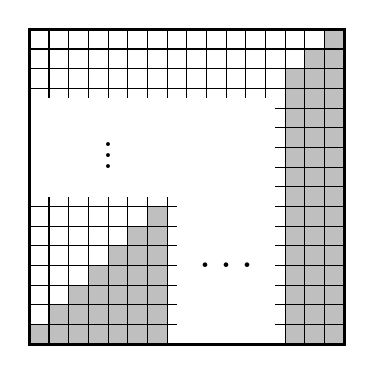
\begin{tikzpicture}[scale=0.5, x=0.5cm, y=0.5cm, font=\LARGE]
        \foreach \x in {0,...,15} 
            \foreach \y in {0,...,15}
                {
                    \pgfmathparse{(\x >= \y && (\x<7 || \x>12)) ? "lightgray" : "white"}
                    \edef\colour{\pgfmathresult}
                    \path[fill=\colour] (\x,\y) rectangle ++ (1,1);
                    \draw[black] (\x,\y) rectangle ++ (1,1);
                }
        \fill[white] (0, 7.5) rectangle ++ (8,5) node[color=black, pos=.5, align=center]{$\vdots$};
        \fill[white] (7.5, 0) rectangle ++ (5,8) node[color=black, pos=.5, align=center]{$\dots$};
        \fill[white] (7.5, 7.5) rectangle ++ (5,5) node[color=black, pos=.5, align=center]{$\iddots$};
        \draw[very thick, black] (0, 0) rectangle ++ (16,16);
    \end{tikzpicture}
\end{center}

现在,要求 $S(n)$ 的公式相当于求正方形内绘制的所有矩形覆盖区域的\emph{面积}。尝试将各个面积相加只是重述了这个问题,因此我们需要想办法将该面积与正方形的总面积联系起来。为此,我们要考虑剩下的是什么;也就是说,我们如何描述未被矩形覆盖的正方形的面积?看一下第一个 $1 \times 1$ 矩形正上方的区域:它也是一个矩形,尺寸为 $(n - 1) \times 1$。

看一下 $2 \times 1$ 矩形上方的区域:它是一个 $(n-2) \times 1$ 矩形。这种模式一直持续!最终,我们在 $(n - 1) \times 1$ 矩形上方有一个 $1 \times 1$ 矩形,并且最后一个 $n \times 1$ 矩形上方没有面积。所有这些矩形的总面积是多少?它看起来很像我们要求的 $S(n)$, 但它只是缺少最后一项 $n$。现在,我们可以将所有矩形的面积与 $S(n)$ 相关联,然后再与正方形面积相关联:
\[n^2 = S(n) + (S(n) - n) = 2S(n) - n\]
因此
\[S(n) = \frac{n^2+n}{2}\]
与我们之前得到的公式相同!

\subsubsection*{解题心得}

有时,有多种方法可以解决问题并得到最终解。有些可能很容易想到,但解起来很麻烦;有些可能很难想到,但解起来很容易;还些可能根本无济于事!通常很难事先判断任何特定方法会发生什么,所以只需动手尝试解题,看看会发生什么就可以了,跟踪你已经尝试过的内容和发生的情况,以便后面可以重新评估该方法。这是我们在数学生涯中需要牢记的一个事实。我们并不总能立即准确地知道该做什么。有时我们难免会陷入困境,或者最终走入死胡同。这不应该令人沮丧;事情就是这样!

作为一个子题,尝试为奇数 $n$ 的情况重做``配对'',但不要忽略求和的最后一项,而是尝试分离中间项并将数字从外到内配对。这是否会得出相同的结果?它看起来比我们使用的方法更容易/更快速/不同吗?或者,如果我们对于某个数字 $k$ 令 $n=2k$ 来处理偶数 $n$ 的情况会怎么样?对于奇数 $n$ 我们又该怎么办?这个符号会改变处理过程吗?会使它变得更容易处理吗? 现在,你能想出任何完全不同的方法来解决这个问题吗? 
